\chapter{Psalm 78}

\begin{figure}
  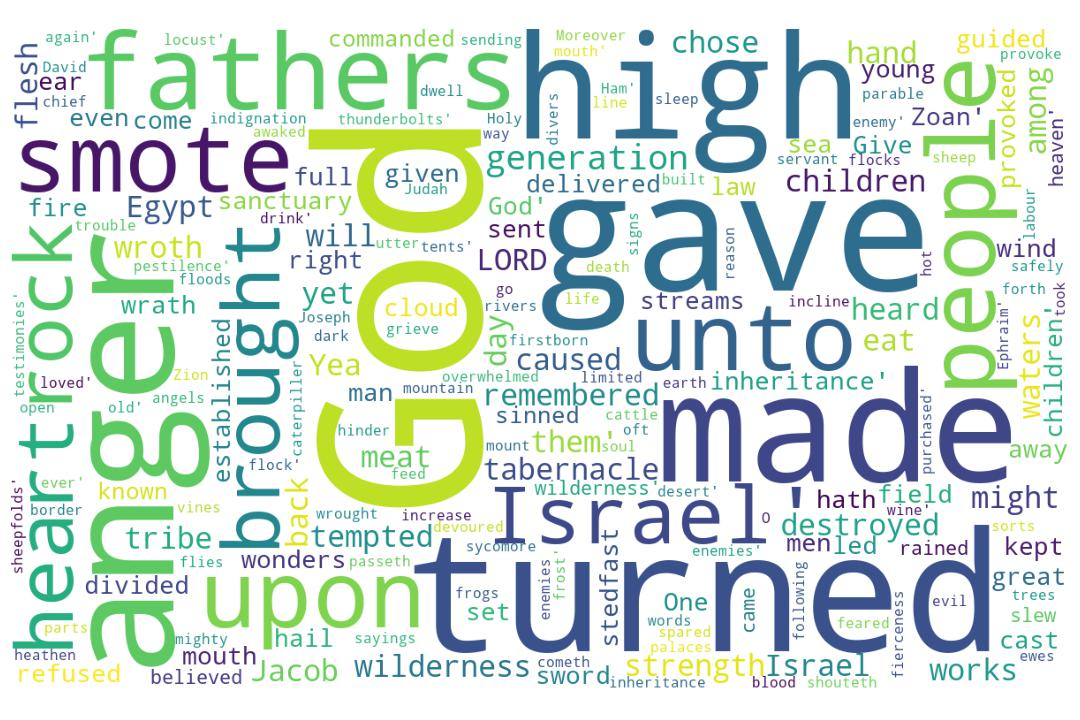
\includegraphics[width=\linewidth]{19OT-Psalms/Psalm78-WordCloud.jpg}
  \caption{Psalm 78 Word Cloud}
  \label{fig:Psalm 78 word Cloud}
\end{figure}

\marginpar{\scriptsize \centering \fcolorbox{bone}{lime}{\textbf{GOD AND HIS PEOPLE}}\\ (Psalm 77) \begin{compactenum}[I.][8]
    \item The  \textbf{Teaching}  \index[scripture]{Psalms!Psa 078:04}(Psa 78:4)
    \item The  \textbf{Testimony}  \index[scripture]{Psalms!Psa 078:05}(Psa 78:5)
    \item The  \textbf{Tempting}  \index[scripture]{Psalms!Psa 078:18}\index[scripture]{Psalms!Psa 078:56} (Psa 78:18, 56)
    \item The  \textbf{Turning}  \index[scripture]{Psalms!Psa 078:41}(Psa 78:41)
    \item The  \textbf{Transgressions}  %\index[scripture]{Psalms!Psa 078:05}(Psalm 78:5)
    \item The  \textbf{Tribe}  \index[scripture]{Psalms!Psa 078:68}(Psa 78:68)
    \item The  \textbf{Tenderness}  \index[scripture]{Psalms!Psa 078:72}(Psa 78:72)
\end{compactenum}}
    




% \textcolor[cmyk]{0.99998,1,0,0}{
\footnote{\textcolor[rgb]{0.00,0.25,0.00}{\hyperlink{TOC}{Return to end of Table of Contents.}}}\footnote{\href{https://audiobible.com/bible/psalms_78.html}{\textcolor[cmyk]{0.99998,1,0,0}{Psalm 78 Audio}}}\textcolor[cmyk]{0.99998,1,0,0}{Maschil of Asaph}\\
\\
\textcolor[cmyk]{0.99998,1,0,0}{Give ear, O my people, \emph{to} my law: incline your ears to the words of my mouth.}
[2] \textcolor[cmyk]{0.99998,1,0,0}{I will open my mouth in a parable: I will utter dark sayings of old:}
[3] \textcolor[cmyk]{0.99998,1,0,0}{Which we have heard and known, and our fathers have told us.}
[4] \textcolor[cmyk]{0.99998,1,0,0}{We will not hide \emph{them} from their children, shewing to the \fcolorbox{bone}{lime}{generation to come} the praises of the LORD, and his strength, and his wonderful works that he hath done.}
[5] \textcolor[cmyk]{0.99998,1,0,0}{For he established a \fcolorbox{bone}{lime}{testimony} in Jacob, and appointed a law in Israel, which he commanded our fathers, that they should make them known to their children:}
[6] \textcolor[cmyk]{0.99998,1,0,0}{That the generation to come might know \emph{them,} \emph{even} the children \emph{which} should be born; \emph{who} should arise and declare \emph{them} to their children:}
[7] \textcolor[cmyk]{0.99998,1,0,0}{That they might set their hope in God, and not forget the works of God, but keep his commandments:}
[8] \textcolor[cmyk]{0.99998,1,0,0}{And might not be as their fathers, a stubborn and rebellious generation; a generation \emph{that} set not their heart aright, and whose spirit was not stedfast with God.}
[9] \textcolor[cmyk]{0.99998,1,0,0}{The children of Ephraim, \emph{being} armed, \emph{and} carrying bows, turned back in the day of battle.}
[10] \textcolor[cmyk]{0.99998,1,0,0}{They kept not the covenant of God, and refused to walk in his law;}
[11] \textcolor[cmyk]{0.99998,1,0,0}{And forgat his works, and his wonders that he had shewed them.}
[12] \textcolor[cmyk]{0.99998,1,0,0}{Marvellous things did he in the sight of their fathers, in the land of Egypt, \emph{in} the field of Zoan.}
[13] \textcolor[cmyk]{0.99998,1,0,0}{He divided the sea, and caused them to pass through; and he made the waters to stand as an heap.}
[14] \textcolor[cmyk]{0.99998,1,0,0}{In the daytime also he led them with a cloud, and all the night with a light of fire.}
[15] \textcolor[cmyk]{0.99998,1,0,0}{He clave the rocks in the wilderness, and gave \emph{them} drink as \emph{out} \emph{of} the great depths.}
[16] \textcolor[cmyk]{0.99998,1,0,0}{He brought streams also out of the rock, and caused waters to run down like rivers.}
[17] \textcolor[cmyk]{0.99998,1,0,0}{And they sinned yet more against him by provoking the most High in the wilderness.}
[18] \textcolor[cmyk]{0.99998,1,0,0}{And they \fcolorbox{bone}{lime}{tempted} God in their heart by asking meat for their lust.}
[19] \textcolor[cmyk]{0.99998,1,0,0}{Yea, they spake against God; they said, Can God furnish a table in the wilderness?}
[20] \textcolor[cmyk]{0.99998,1,0,0}{Behold, he smote the rock, that the waters gushed out, and the streams overflowed; can he give bread also? can he provide flesh for his people?}
[21] \textcolor[cmyk]{0.99998,1,0,0}{Therefore the LORD heard \emph{this}, and was wroth: so a fire was kindled against Jacob, and anger also came up against Israel;}
[22] \textcolor[cmyk]{0.99998,1,0,0}{Because they believed not in God, and trusted not in his salvation:}
[23] \textcolor[cmyk]{0.99998,1,0,0}{Though he had commanded the clouds from above, and opened the doors of heaven,}
[24] \textcolor[cmyk]{0.99998,1,0,0}{And had rained down manna upon them to eat, and had given them of the corn of heaven.}
[25] \textcolor[cmyk]{0.99998,1,0,0}{Man did eat angels' food: he sent them meat to the full.}
[26] \textcolor[cmyk]{0.99998,1,0,0}{He caused an east wind to blow in the heaven: and by his power he brought in the south wind.}
[27] \textcolor[cmyk]{0.99998,1,0,0}{He rained flesh also upon them as dust, and feathered fowls like as the sand of the sea:}
[28] \textcolor[cmyk]{0.99998,1,0,0}{And he let \emph{it} fall in the midst of their camp, round about their habitations.}
[29] \textcolor[cmyk]{0.99998,1,0,0}{So they did eat, and were well filled: for he gave them their own desire;}
[30] \textcolor[cmyk]{0.99998,1,0,0}{They were not estranged from their lust. But while their meat \emph{was} yet in their mouths,}
[31] \textcolor[cmyk]{0.99998,1,0,0}{The wrath of God came upon them, and slew the fattest of them, and smote down the chosen \emph{men} of Israel.}
[32] \textcolor[cmyk]{0.99998,1,0,0}{For all this they sinned still, and believed not for his wondrous works.}
[33] \textcolor[cmyk]{0.99998,1,0,0}{Therefore their days did he consume in vanity, and their years in trouble.}
[34] \textcolor[cmyk]{0.99998,1,0,0}{When he slew them, then they sought him: and they returned and enquired early after God.}
[35] \textcolor[cmyk]{0.99998,1,0,0}{And they remembered that God \emph{was} their rock, and the high God their redeemer.}
[36] \textcolor[cmyk]{0.99998,1,0,0}{Nevertheless they did flatter him with their mouth, and they lied unto him with their tongues.}
[37] \textcolor[cmyk]{0.99998,1,0,0}{For their heart was not right with him, neither were they stedfast in his covenant.}
[38] \textcolor[cmyk]{0.99998,1,0,0}{But he, \emph{being} full of compassion, forgave \emph{their} iniquity, and destroyed \emph{them} not: yea, many a time turned he his anger away, and did not stir up all his wrath.}
[39] \textcolor[cmyk]{0.99998,1,0,0}{For he remembered that they \emph{were} \emph{but} flesh; a wind that passeth away, and cometh not again.}
[40] \textcolor[cmyk]{0.99998,1,0,0}{How oft did they provoke him in the wilderness, \emph{and} grieve him in the desert!}
[41] \textcolor[cmyk]{0.99998,1,0,0}{Yea, they \fcolorbox{bone}{lime}{turned} back and tempted God, and limited the Holy One of Israel.}
[42] \textcolor[cmyk]{0.99998,1,0,0}{They remembered not his hand, \emph{nor} the day when he delivered them from the enemy.}
[43] \textcolor[cmyk]{0.99998,1,0,0}{How he had wrought his signs in Egypt, and his wonders in the field of Zoan:}
[44] \textcolor[cmyk]{0.99998,1,0,0}{And had turned their rivers into blood; and their floods, that they could not drink.}
[45] \textcolor[cmyk]{0.99998,1,0,0}{He sent divers sorts of flies among them, which devoured them; and frogs, which destroyed them.}
[46] \textcolor[cmyk]{0.99998,1,0,0}{He gave also their increase unto the caterpiller, and their labour unto the locust.}
[47] \textcolor[cmyk]{0.99998,1,0,0}{He destroyed their vines with hail, and their sycomore trees with frost.}
[48] \textcolor[cmyk]{0.99998,1,0,0}{He gave up their cattle also to the hail, and their flocks to hot thunderbolts.}
[49] \textcolor[cmyk]{0.99998,1,0,0}{He cast upon them the fierceness of his anger, wrath, and indignation, and trouble, by sending evil angels \emph{among} \emph{them}.}
[50] \textcolor[cmyk]{0.99998,1,0,0}{He made a way to his anger; he spared not their soul from death, but gave their life over to the pestilence;}
[51] \textcolor[cmyk]{0.99998,1,0,0}{And smote all the firstborn in Egypt; the chief of \emph{their} strength in the tabernacles of Ham:}
[52] \textcolor[cmyk]{0.99998,1,0,0}{But made his own people to go forth like sheep, and guided them in the wilderness like a flock.}
[53] \textcolor[cmyk]{0.99998,1,0,0}{And he led them on safely, so that they feared not: but the sea overwhelmed their enemies.}
[54] \textcolor[cmyk]{0.99998,1,0,0}{And he brought them to the border of his sanctuary, \emph{even} \emph{to} this mountain, \emph{which} his right hand had purchased.}
[55] \textcolor[cmyk]{0.99998,1,0,0}{He cast out the heathen also before them, and divided them an inheritance by line, and made the tribes of Israel to dwell in their tents.}
[56] \textcolor[cmyk]{0.99998,1,0,0}{Yet they \fcolorbox{bone}{lime}{tempted} and provoked the most high God, and kept not his testimonies:}
[57] \textcolor[cmyk]{0.99998,1,0,0}{But turned back, and dealt unfaithfully like their fathers: they were turned aside like a deceitful bow.}
[58] \textcolor[cmyk]{0.99998,1,0,0}{For they provoked him to anger with their high places, and moved him to jealousy with their graven images.}
[59] \textcolor[cmyk]{0.99998,1,0,0}{When God heard \emph{this}, he was wroth, and greatly abhorred Israel:}
[60] \textcolor[cmyk]{0.99998,1,0,0}{So that he forsook the tabernacle of Shiloh, the tent \emph{which} he placed among men;}
[61] \textcolor[cmyk]{0.99998,1,0,0}{And delivered his strength into captivity, and his glory into the enemy's hand.}
[62] \textcolor[cmyk]{0.99998,1,0,0}{He gave his people over also unto the sword; and was wroth with his inheritance.}
[63] \textcolor[cmyk]{0.99998,1,0,0}{The fire consumed their young men; and their maidens were not given to marriage.}
[64] \textcolor[cmyk]{0.99998,1,0,0}{Their priests fell by the sword; and their widows made no lamentation.}
[65] \textcolor[cmyk]{0.99998,1,0,0}{Then the Lord awaked as one out of sleep, \emph{and} like a mighty man that shouteth by reason of wine.}
[66] \textcolor[cmyk]{0.99998,1,0,0}{And he smote his enemies in the hinder parts: he put them to a perpetual reproach.}
[67] \textcolor[cmyk]{0.99998,1,0,0}{Moreover he refused the tabernacle of Joseph, and chose not the tribe of Ephraim:}
[68] \textcolor[cmyk]{0.99998,1,0,0}{But chose the \fcolorbox{bone}{lime}{tribe} of Judah, the mount Zion which he loved.}
[69] \textcolor[cmyk]{0.99998,1,0,0}{And he built his sanctuary like high \emph{palaces}, like the earth which he hath established for ever.}
[70] \textcolor[cmyk]{0.99998,1,0,0}{He chose David also his servant, and took him from the sheepfolds:}
[71] \textcolor[cmyk]{0.99998,1,0,0}{From following the ewes great with young he brought him to feed Jacob his people, and Israel his inheritance.}
[72] \textcolor[cmyk]{0.99998,1,0,0}{So he fed them according to the integrity of his heart; and guided them by the \fcolorbox{bone}{lime}{skilfulness} of his hands.}